\documentclass{../base/base}
% Dateikodierung ist utf8
\usepackage[utf8]{inputenc}
\usepackage{url}
\usepackage[export]{adjustbox}
\usepackage{amsmath}
\usepackage{listings}
\usepackage{tikz}
\usepackage{tabularx}
\usepackage{color,colortbl}
\usepackage{ulem}
\usepackage{pdfpages}
\usepackage{ wasysym }
\usepackage{ booktabs }
\usepackage{lscape}
\usepackage{multicol}

\begin{document}

\Abgabeblatt{Assignment 2}{23.03.2018}{????}{????}{Yannis Rohloff (yannis@uni-bremen.de)}{Liu Meng(lium@uni-bremen.de)}{Peter Tschubij (tschupet@uni-bremen.de)}

\lstset{
    language=Python,
    basicstyle=\ttfamily\small,
    aboveskip={1.0\baselineskip},
    belowskip={1.0\baselineskip},
    columns=fixed,
    extendedchars=true,
    breaklines=true,
    tabsize=4,
    prebreak=\raisebox{0ex}[0ex][0ex]{\ensuremath{\hookleftarrow}},
    frame=lines,
    showtabs=false,
    showspaces=false,
    showstringspaces=false,
    keywordstyle=\color[rgb]{0.627,0.126,0.941},
    commentstyle=\color[rgb]{0.133,0.545,0.133},
    stringstyle=\color[rgb]{01,0,0},
    numbers=left,
    numberstyle=\small,
    stepnumber=1,
    numbersep=10pt,
    captionpos=t,
    escapeinside={\%*}{*)}
}


\section*{Exercise 1: Circuit Equivalence}


We first defined all 4 logical expressions in a general way via four python functions. We then manually associate the neccesary variables with numbers and call the defined functions. \\
Last, we verify the equivaleny.

% code
\lstinputlisting[label={list:circ},caption=Python code to generate DIMACS CNF]{liu_circuit.py}

\lstinputlisting[label={list:cnf},caption=Generated DIMACS compatible CNF]{liu_circuit.cnf}

\lstinputlisting[label={list:solution},caption=Picosat output]{liu_circuit.solution}

There is no assignment given by picosat so there is no assignment for A,B,C for which the outputs of both circuits are different, therefore the circuits are equivalent.

\section*{Problem 2:  DPLL without unit propagation}
Variables $V = \{v_1,v_2...v_n\}$ in boolean formula (general form):
%\begin{equation*}
\begin{multline*}
    \psi(v_1,v_2...v_n) = (v_1\lor v_2\lor v_3...\lor v_n)\land (v_2\lor v_3...\lor v_n)...\land (v_n) \\
    \land(v_{n-1} \lor \neg v_n) \land (v_{n-2}\lor \neg v_{n-1}\lor \neg v_n)...	\land (v_1\lor \neg v_2...\lor \neg v_n)
\end{multline*}
%\end{equation*}
The first line builds clauses that allow the algorithm to assign false to every variable.
As soon as the last variable is set to false the clause $(v_n)$ is falsified.
After $v_n$ is set to true a clause in the second row will be falsified.
Then $v_{n-1}$ is set to true and $v_n$ to false again. This contradicts again. This continues until all variables are true. (As seen in the drawings on the last page).

If we use the order $\{v_1,v_2,\dots,v_n\}$, the Algorithm 1 will generate $$\sum_{i=1}^{n} 2^{i} $$ nodes to search the correct answer. 

But if we use the order $\{v_n, v_n-1,\dots,v_2, v_1\}$, it will only use $2\cdot n$ nodes to complete. 
It starts by setting $v_n$ to false and immediately falsifies clause $v_n$. $v_n$ is then set to true.
$v_{n-1}$ will be set to false next but also causes a violated clause so it is set to true immedialty, too.
The same goes on for the other variables until they are all true.

The following graphs for $n=4$ show the difference.
\clearpage
\begin{centering}
    The formula:
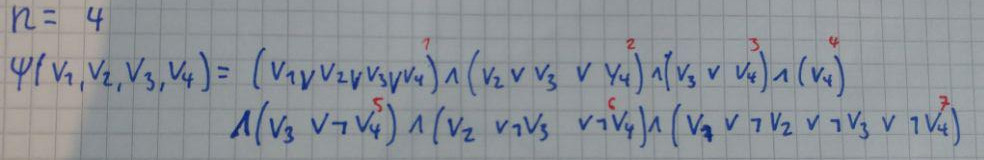
\includegraphics[width=0.9\textwidth]{def.jpg} \\
With increasing index:
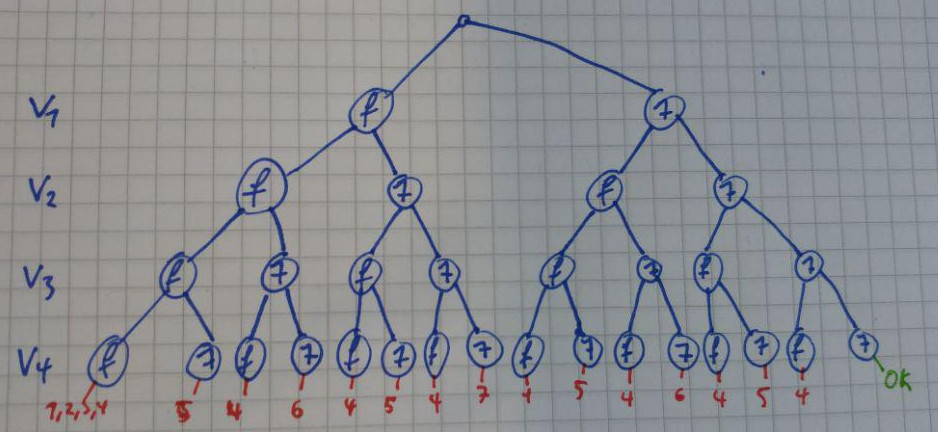
\includegraphics[width=0.9\textwidth]{forward.jpg} \\
With decreasing index:
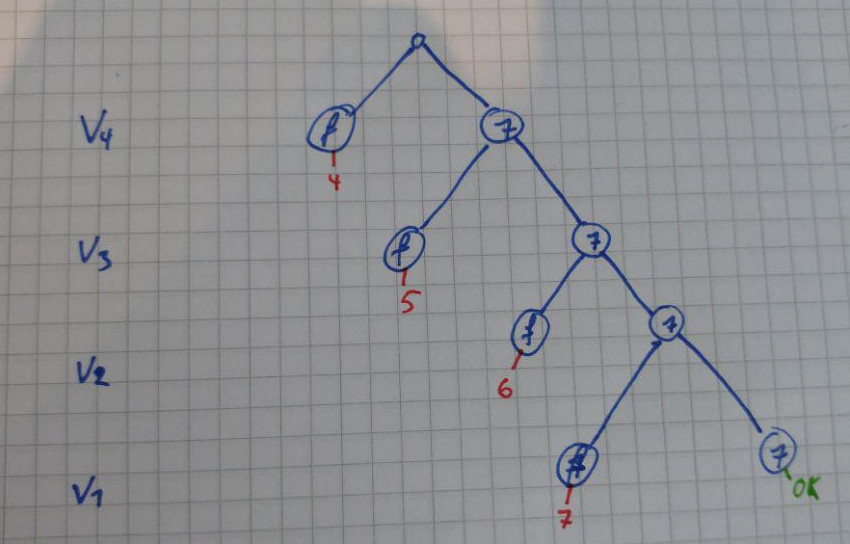
\includegraphics[width=0.9\textwidth]{backward.jpg} \\
\end{centering}




\end{document}
